\documentclass[11pt]{article}
\usepackage[margin=1in]{geometry}
\usepackage{amsmath,amssymb}
\usepackage{graphicx}
\usepackage{booktabs}
\usepackage{hyperref}
\usepackage{xcolor}

\title{Sensitivity Analysis of the Roundabout DQN Policy}
\author{Stanford Roundabout Project}
\date{\today}

\begin{document}
\maketitle

\section{Explainability}

We performed two kinds of sensitivity analysis on our roundabout DQN policy,
following Algorithms~11.1 and~11.4 in \emph{Verification and Validation for
Safety-Critical Systems}~\cite{kochenderfer2025val}. The first analysis studies
\textbf{scenario-level} parameters (e.g., other vehicles' speed, initial
conditions). The second analysis focuses on a \textbf{single failure
trajectory} and asks which timesteps contribute most to the robustness of that
trajectory, both in a local (sensitivity) and interaction-aware (Shapley)
sense.

\subsection{Scenario-Level Sensitivity}

Let $p$ denote a scalar scenario parameter (for example, the mean speed of
background vehicles) and let $r(p)$ denote the average robustness of the
resulting rollouts under the learned policy. Following the textbook's
discussion of one-at-a-time sensitivity analysis, we vary a single parameter
over a grid $\{p_1,\dots,p_K\}$ while holding all other parameters at their
nominal values, and estimate a scalar sensitivity score by the sample standard
deviation
\begin{equation}
    \sigma(p)
    \;=\;
    \sqrt{
      \frac{1}{K-1}
      \sum_{k=1}^K
        \bigl(r(p_k) - \bar r\bigr)^2
    },
    \qquad
    \bar r = \frac{1}{K}\sum_{k=1}^K r(p_k).
\end{equation}
Intuitively, $\sigma(p)$ is large when changing $p$ produces large changes in
robustness, so we use it to rank parameters by global influence.

For each parameter we swept a range of values, ran $30$ rollouts per value, and
estimated $r(p_k)$ by the mean robustness over those rollouts. Robustness and
failure rate both change as we move each parameter. Using $\sigma(p)$ as the
sensitivity score, the ranking was:

\begin{table}[h]
    \centering
    \caption{Parameter Sensitivity and Max Fail Rate}
    \begin{tabular}{clcc}
    \hline
    \textbf{Rank} & \textbf{Parameter} & \textbf{Sensitivity} & \textbf{Max Fail Rate} \\
    \hline
    1 & other\_vehicle\_speed & 0.1489 & 63.3\% \\
    2 & entering\_vehicle\_mu & 0.1028 & 46.7\% \\
    3 & initial\_speed\_mu    & 0.0929 & 20.0\% \\
    4 & ctrl\_noise\_p        & 0.0779 & 16.7\% \\
    \hline
    \end{tabular}
    \label{tab:sensitivity_rankings}
\end{table}

\begin{figure}[h]
    \centering
    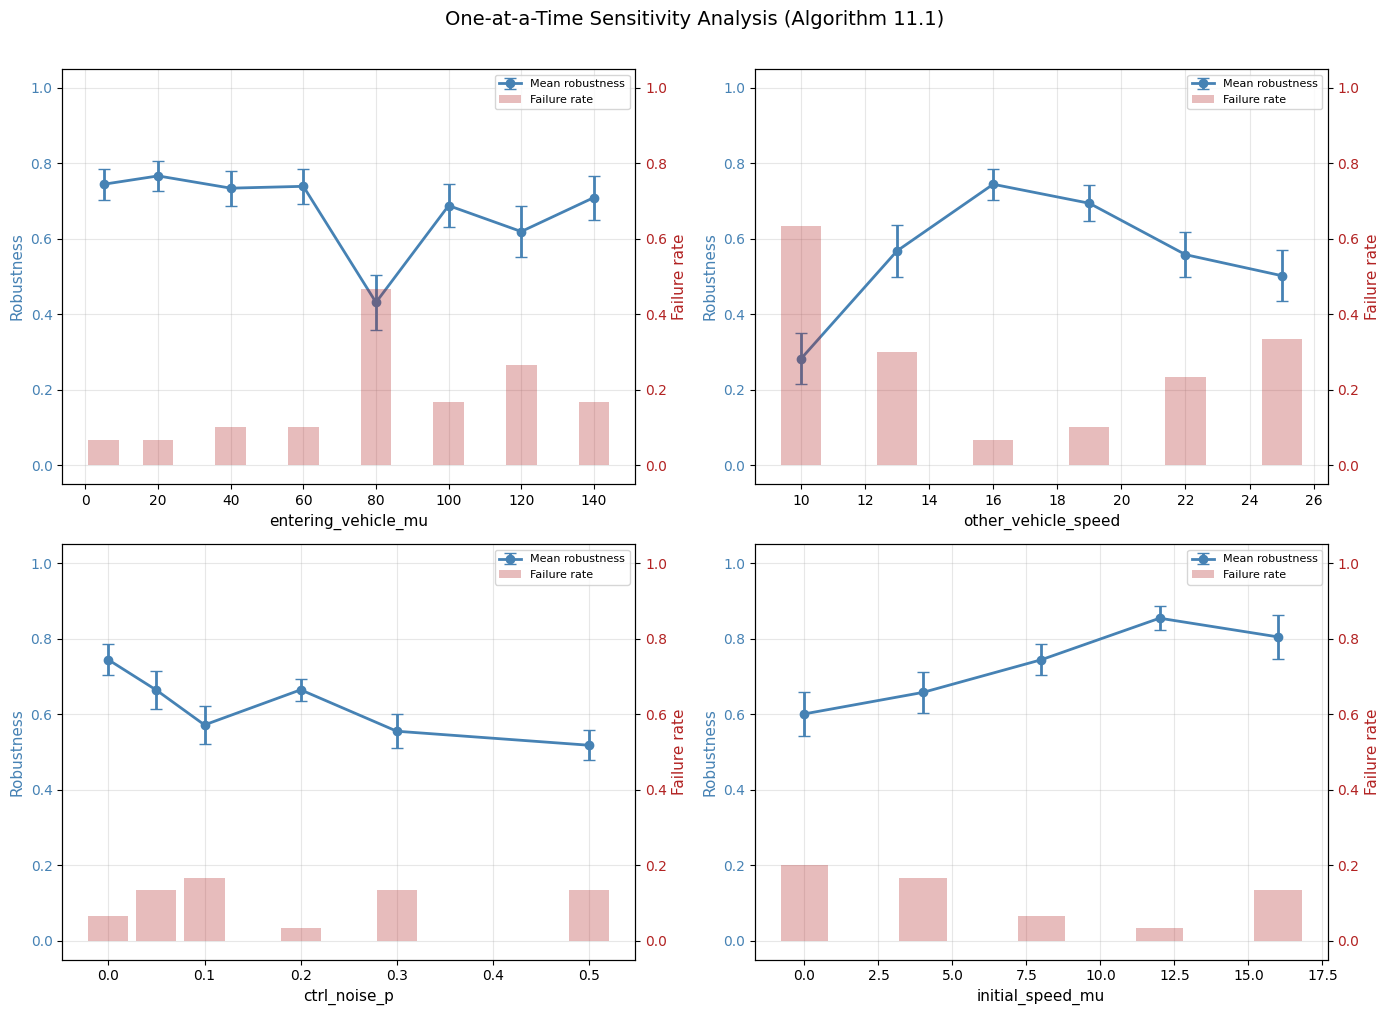
\includegraphics[width=0.9\linewidth]{figures/One-at-a-Time_Sensitivity.png}
    \caption{One at a time sensitivity}
    \label{fig:sensitivity}
\end{figure}

\subsection{Per-Timestep Sensitivity}

Consider a fixed reference rollout (trajectory) $\tau$ produced by the policy,
with robustness $r(\tau)$. Let $\tau^{(t,i)}$ denote a perturbed trajectory in
which only the discrete action at timestep $t$ has been changed (to some
admissible alternative in $\mathcal{A}_t^{(i)}$), and the rest of the rollout is
replayed deterministically. Following Algorithm~11.1, we approximate the
sensitivity of robustness at timestep $t$ by
\begin{equation}
    s_t
    \;\approx\;
    \operatorname{std}\Bigl(
        \bigl|
            r(\tau^{(t,1)}) - r(\tau)
        \bigr|,
        \dots,
        \bigl|
            r(\tau^{(t,M)}) - r(\tau)
        \bigr|
    \Bigr),
\end{equation}
where the set of perturbations $\{\tau^{(t,1)},\dots,\tau^{(t,M)}\}$ ranges
over the admissible discrete actions at timestep $t$ (excluding the reference
action). In our implementation, the action space is finite---SLOWER, FASTER,
LANE\_LEFT, IDLE, and LANE\_RIGHT---so instead of sampling we enumerate all
admissible alternatives at $t$ and evaluate $s_t$ over this finite set. Large
$s_t$ means that small local changes to the action at $t$ tend to produce large
changes in robustness.

Empirically, the maximum sensitivity occurs at timestep $t=0$ (score
$0.1745$), indicating that the very first action in this failure run has the
largest local effect on robustness; early decisions in the episode are
especially critical for this trajectory.

\subsection{Per-Timestep Shapley Values}

Sensitivity treats each timestep independently. To capture interaction effects
between timesteps, we use Shapley values, following the feature importance
definition in Section~11.3.2 of the textbook. Let the index set of timesteps be
$I = \{1,\dots,T\}$ and let $f(\mathbf{a}) = r(\tau(\mathbf{a}))$ denote the
robustness as a function of the full action sequence
$\mathbf{a} = (a_1,\dots,a_T)$. For any subset $S \subseteq I$, define
the conditional expectation
\begin{equation}
  f_S(\mathbf{a})
  = \mathbb{E}\bigl[f(\mathbf{a}') \mid a'_t = a_t \;\text{for all}\; t \in S\bigr],
\end{equation}
that is, the expected robustness when we fix the actions in $S$ to their
reference values and sample the remaining actions from the nominal trajectory
distribution.

The Shapley value $\phi_t(\mathbf{a})$ of timestep $t$ is then defined as the
average marginal contribution of including $t$ in all possible subsets:
\begin{equation}
  \phi_t(\mathbf{a})
  =
  \sum_{S \subseteq I \setminus \{t\}}
   \frac{|S|!\,(T-|S|-1)!}{T!}
   \Bigl(
     f_{S \cup \{t\}}(\mathbf{a}) - f_S(\mathbf{a})
   \Bigr).
  \label{eq:shapley-def}
\end{equation}
Equivalently, letting $\mathcal{P}(T)$ be the set of all permutations of the
indices $\{1,\dots,T\}$, the Shapley value can be written as
\begin{equation}
  \phi_t(\mathbf{a})
  =
  \frac{1}{T!}
  \sum_{\pi \in \mathcal{P}(T)}
    \Bigl(
      f_{\pi_{1:j}}(\mathbf{a}) - f_{\pi_{1:j-1}}(\mathbf{a})
    \Bigr),
  \qquad
  j = \text{position of } t \text{ in permutation } \pi,
  \label{eq:shapley-perm}
\end{equation}
where $\pi_{1:j}$ denotes the first $j$ indices in the permutation $\pi$.

Exactly computing~\eqref{eq:shapley-def} or~\eqref{eq:shapley-perm} is
intractable for long trajectories, so we follow Algorithm~11.4 and approximate
$\phi_t$ using Monte Carlo sampling. For each timestep $t$ we:
\begin{enumerate}
  \item Sample $M=20$ disturbance trajectories and permutations of the indices.
  \item For each sample, construct two rollouts: one in which we use the
        reference action $a_t$ at timestep $t$ and one in which we replace
        $a_t$ by a nominally sampled action (with the rest of the actions
        determined by the sampled permutation).
  \item Take the robustness difference $\Delta r$ between the two rollouts as
        that sample's marginal contribution of timestep $t$.
  \item Average the $\Delta r$ values over samples to obtain $\phi_t$.
\end{enumerate}

By construction, a positive Shapley value $\phi_t$ indicates that the reference
action at timestep $t$ tends to \emph{increase} robustness relative to
plausible counterfactual actions, while a negative value indicates that it
tends to \emph{decrease} robustness.

In our failure trajectory, both the sensitivity scores $\{s_t\}$ and the
Shapley values $\{\phi_t\}$ agree that timestep $t=0$ is the most important.
Several later FASTER actions (around $t \in \{6,7,9\}$) and an early IDLE
action ($t=2$) also have relatively large $|\phi_t|$. The trajectory plot of
minimum distance versus time, with sensitivities and Shapley values overlaid in
the style of Figures~11.5 and~11.9 of the textbook, highlights these timesteps
as the main contributors to the failure.

\begin{figure}[h]
    \centering
    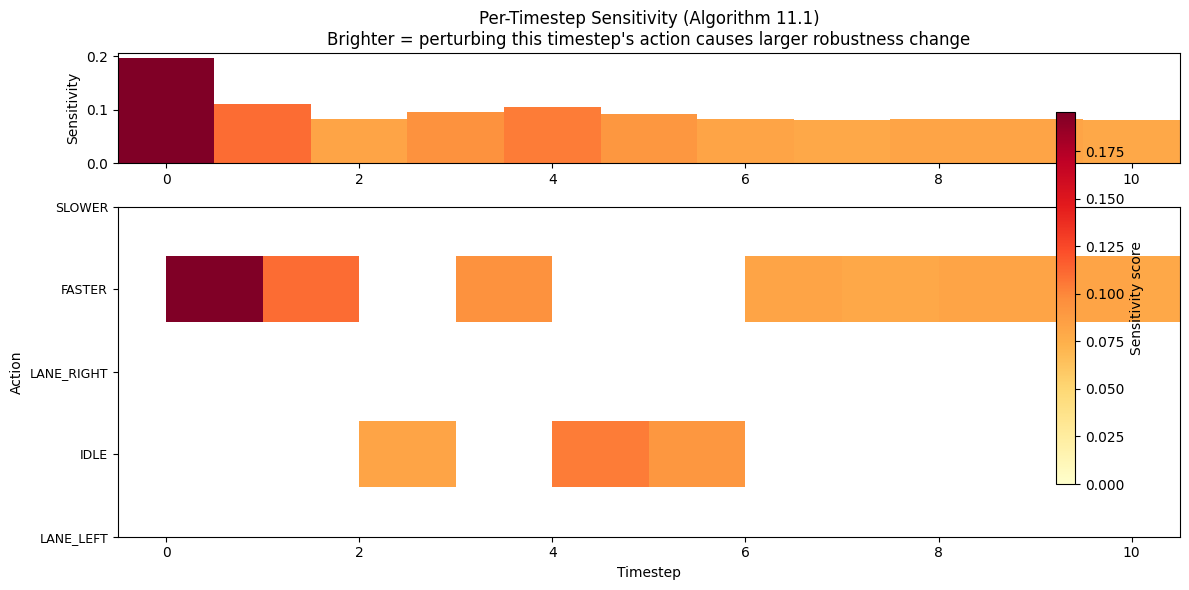
\includegraphics[width=1\linewidth]{figures/Per-Timestep_Sensitivity.png}
    \caption{Per-timestep sensitivity (Algorithm 11.1) and Shapley values
             (Algorithm 11.4) for a single failure trajectory. The black line
             shows minimum distance over time, the red band indicates the
             collision region, and colored markers indicate importance at each
             timestep.}
    \label{fig:per-timestep}
\end{figure}

\bibliographystyle{plain}
\bibliography{references}
\end{document}
